\documentclass{abnt-UTFPR}                                          % estilo de documento abnTeX
\usepackage[alf,abnt-emphasize=bf,bibjustif,recuo=0cm]{abntcite}    % estilo de bibliografia abnTeX
\usepackage[brazil]{babel}                                          % pacote portugues brasileiro
\usepackage[latin1]{inputenc}                                       % pacote para acentuacao direta
\usepackage{amsmath,amsfonts,amssymb}                               % pacote matematico
\usepackage{graphicx}                                               % pacote grafico
\usepackage{times}                                                  % fonte times
\usepackage{verbatim}                                               % multi-line comment

% ---------- Preambulo ----------
\instituicao{Universidade Tecnol�gica Federal do Paran�} % nome da instituicao
\departamento{Departamento Acad�mico de Inform�tica} % nome do departamento
\programa{Bacharelado em Engenharia de Computa��o} % nome do curso

\documento{Trabalho de Conclus�o de Curso} % [Trabalho de Conclus\~ao de Curso] ou [Relat\'orio de Est\'agio]
\titulacao{Engenheiro} % [T\'ecnico], [Tecn\'ologo] ou [Engenheiro]

\titulo{An�lise Qualitativa de Algoritmos de Navega��o Fuzzy} % titulo do trabalho em portugues
\title{Qualitative Analysis of Fuzzy Algorithms} % titulo do trabalho em ingles

\autor{Alexandre Jacques Marin} % primeiro autor do trabalho
\autordois{J�lio Cesar Nardelli Borges} % segundo autor do trabalho, caso exista
\autortres{Yuri Antin Wergrzn} % terceiro autor do trabalho, caso exista
%\autorquatro{Nome do Quarto Autor} % quarto autor do trabalho, caso exista
\cita{MARIN, Alexandre; BORGES, J�lio; WERGRZN, Yuri } % sobrenome (maiusculas) e nome do(s) autor(es) do trabalho, separados por ponto-e-virgula (ate quatro autores para TCC)

\palavraschave{Navega��o, Fuzzy, Rob�s, Aut�noma, ...} % palavras-chave do trabalho
\keywords{Navigation, Fuzzy, Robots, Autonomous, ...} % palavras-chave do trabalho em ingles

\comentario{\UTFPRdocumentodata\ apresentado ao \UTFPRdepartamentodata\ como requisito parcial para obten\c{c}\~ao do grau de \UTFPRtitulacaodata\ no \UTFPRprogramadata\ da \ABNTinstituicaodata.}

\orientador{Jo�o Alberto Fabro} % nome do orientador do trabalho
%\orientador[Orientadora:]{Nome da Orientadora} % <- no caso de orientadora, usar esta sintaxe
\coorientador{Heitor Silv�rio Lopes} % nome do co-orientador do trabalho, caso exista
%\coorientador[Co-orientadora:]{Nome da Co-orientadora} % <- no caso de co-orientadora, usar esta sintaxe

\local{Curitiba} % cidade
\data{2012} % ano


%---------- Inicio do Documento ----------
\begin{document}

\capa % geracao automatica da capa
\folhaderosto % geracao automatica da folha de rosto
%\termodeaprovacao % <- ainda a ser implementado corretamente

% dedicat�ria (opcional)
\begin{dedicatoria}
Texto da dedicat\'oria.
\end{dedicatoria}

% agradecimentos (opcional)
\begin{agradecimentos}
Texto dos agradecimentos.
\end{agradecimentos}

% epigrafe (opcional)
\begin{epigrafe}
Texto da ep\'igrafe.
\end{epigrafe}

%resumo
\begin{resumo}
Este documento descreve detalhadamente a execu��o do projeto \"An�lise Qualitativa de Algoritmos de Navega��o Fuzzy\", feito como trabalho de conclus�o de curso de Engenharia de Computa��o na Universidade Tecnol�gica Federal do Paran�.
\end{resumo}

%abstract
\begin{abstract}
Abstract text (maximum of 500 words).
\end{abstract}

% listas (opcionais, mas recomenda-se a partir de 5 elementos)
\listadefiguras % geracao automatica da lista de figuras
\listadetabelas % geracao automatica da lista de tabelas
\listadesiglas % geracao automatica da lista de siglas
\listadesimbolos % geracao automatica da lista de simbolos

% sumario
\sumario % geracao automatica do sumario


%---------- Primeiro Capitulo ----------
\chapter{Introdu��o}

O problema do controle de navega��o de rob�s m�veis aut�nomos �
um campo da Engenharia da Computa��o que representa um grande
desafio, devido ao fato de o ambiente ser din�mico, haver sensoriamento
sujeito a ru�dos e exig�ncias de controle e tomada de decis�o em tempo
real. Um sistema de navega��o deve garantir que o rob� m�vel atinja
satisfatoriamente o destino de sua trajet�ria, enviando ao rob� comandos
necess�rios para locomo��o, de maneira precisa e suave, ao mesmo
tempo em que permite rea��es r�pidas �s mudan�as de ambiente para
evitar colis�es \cite{FRACASSO}.

O presente trabalho � um estudo comparativo entre dois algoritmos de navega��o,
que ser�o implementados em um rob� m�vel aut�nomo o qual dever� desviar obst�culos. 
Um dos algoritmos � uma implementa��o utilizando l�gica fuzzy, com tomada de decis�o
baseada diretamente em regras fuzzy, enquanto que o outro � um algoritmo 
baseado em FCM (Fuzzy Cognitive Maps).

\section{Motiva��o}

Ao realizar uma pesquisa para an�lise do estado da arte, percebeu-se a 
exist�ncia de trabalhos que apresentam novos m�todos para navega��o 
aut�noma atrav�s do uso de l�gica fuzzy, entretanto,
s�o poucos os trabalhos propondo a compara��o entre os m�todos j� existentes.
Com o intuito de enriquecer essa �rea de pesquisa, a equipe optou por
desenvolver este projeto, que representa um ramo de elevado valor acad�mico.
Para realizar a compara��o pr�tica destes algoritmos, o uso de uma
plataforma rob�tica real determinou obten��o a obten��o de resultados mais significativos pois
os algoritmos foram executados em condi��es reais. 

A plataforma foi obtida atrav�s da reconstru��o e 
adapta��o do "Bellator", o qual era um rob� m�vel que esteve em constru��o em um projeto 
da disciplina de Oficinas de Integra��o 3 \cite{BELLATOR}. Teve-se em vista o 
custo elevado de plataformas rob�ticas m�veis, como por exemplo, a X80, cujo 
pre�o � de 2795 d�lares \cite{X80}, ao decidir entre adquirir uma plataforma 
comercial ou reconstruir e adequar o Bellator. A possibilidade de disponibilizar
a plataforma reconstru�da para trabalhos acad�micos futuros tamb�m foi levada
em considera��o nesse projeto. 

Os algoritmos escolhidos s�o um algoritmo baseado em logica fuzzy, que
foi abordada no curso de gradua��o e pode ser aplicada em navega��o rob�tica e um 
algoritmo baseado em FCM, o qual era uma metodologia desconhecida pelos membros da equipe mas com a qual
surgiu a oportunidade de desenvolver esse trabalho.

\section{Objetivos}

Os objetivos do presente trabalho s�o a reconstru��o e adequa��o do rob� Bellator, a descri��o do hardware e software do mesmo ap�s essa tarefa, a implementa��o dos algoritmos de navega��o e a execu��o do experimento nos quais estes ser�o comparados. O rob� reconstru�do e adequado dever� ser equipado com sensores de dist�ncia e encoders nas rodas, deve ser alimentado atrav�s de baterias que forne�am adequadamente energia ao sistema microcontrolado, sensores e motores, deve ser capaz de ajustar a velocidade de cada roda de maneira independente, deve processar os sinais dos sensores de dist�ncia e dos encoders e implementar rotinas para disponibilizar esses dados. 

Os algoritmos de navega��o devem ser executados em um hardware acoplado � plataforma, visando reduzir atrasos de comunica��o. Esse hardware dever� ser capaz de ler os dados dos sensores do rob�, como fonte de dados para os algoritmos, e enviar comandos de movimenta��o ao mesmo. Os testes dos algoritmos devem ser realizados em um ambiente igual para ambos sendo que  o objetivo de cada algoritmo � guiar o rob� no deslocamento, desviando-se de poss�veis obst�culos e tendo como entradas, valores de leitura dos sensores e encoders e como sa�da, velocidade e/ou dire��o do rob�.

\section{Metodologia}
A metodologia deste trabalho foi dividida em quatro etapas: reconstru��o e adequa��o do rob� Bellator, estudo, implementa��o e testes dos algoritmos de navega��o. A reconstru��o e adequa��o consistiram na avalia��o do estado do rob�, o projeto e implementa��o do hardware e software necess�rios para o funcionamento adequado do mesmo. Durante a avalia��o, foram testados os sensores de dist�ncia, os encoders das rodas, baterias, motores e as pontes H. A elabora��o do hardware consistiu na confec��o de uma placa de roteamento para alimentar os sensores e encoders, tratar os sinais dos enconders amplificando-os, rotear os sinais dos sensores de dist�ncia, encoders aos respectivos pinos de entrada do microcontrolador e os sinais de PWM gerados por este �s respectivas pontes H do rob�. O software consistiu na adequa��o do firmware previamente dispobilizado no projeto Bellator \cite{BELLATOR}, nas quais as rotinas de leitura dos sensores, comunica��o de dados, recep��o de comandos de controle do rob� e protocolo de comunica��o foram atualizadas de acordo com as necessidades desse projeto. O hardware acoplado � plataforma foi configurado para comunicar-se com o microcontrolador e executar os algoritmos de navega��o. 

O estudo dos algortimos de navega��o consistiu na revis�o bibliogr�fica das abordagens fuzzy e FCM, a implementa��o consistiu na elabora��o dos c�digos na linguagem C++ e compilados para executarem no hardware acoplado e os testes consistiram no rob� guiando-se de forma aut�noma em um ambiente com obst�culos.

\section{Apresenta��o do Documento}

O relat�rio desse trabalho de conclus�o de curso est� dividido em seis cap�tulos: o primeiro corresponde � introdu��o, na qual s�o apresentadas a motiva��o, os objetivos e a metodologia desse projeto. O segundo cap�tulo � a fundamenta��o te�rica do projeto, em que s�o apresentados o estado inicial e o estado final do rob� ap�s a reconstru��o, a explica��o da L�gica Fuzzy e da abordagem FCM. O terceiro cap�tulo � o desenvolvimento do trabalho, no qual s�o descritas as atividades realizadas pela equipe, incluindo a reconstru��o e adequa��o do rob�, o projeto e a implementa��o dos algoritmos. O quarto cap�tulo corresponde aos resultados, que descrevem os testes realizados e os dados obtidos. O quinto cap�tulo � a conclus�o do projeto e o sexto lista as refer�cias bibliograficas.


\chapter{Fundamenta��o Te�rica}
\label{chap:fundteor}

Este cap�tulo apresentar� a fundamenta��o te�rica desse trabalho de conclus�o de curso. Ser�o descritos o estado inicial do projeto e do rob� Bellator, com uma vis�o geral deste ao ser entregue � equipe, a especifica��o do rob� ap�s a reconstru��o, a apresenta��o da L�gica Fuzzy e da metodologia de Mapas Cognitivos Fuzzy (FCM).

%---------- Estado inicial do Projeto ----------
\section{Estado Inicial do Projeto} \label{sec:estpro}

Esta se��o visa descrever com quais recursos a equipe iniciou a execu��o do trabalho, ou seja, a situa��o do rob� e seus componentes de hardware, o principal e mais importante recurso material desse projeto, os componentes de software e a documenta��o de ambos, da forma como foram entregues � equipe.

\subsection{Vis�o Geral}

O rob� disponibilizado � equipe para a realiza��o desse trabalho, o Bellator, � resultado de um projeto n�o conclu�do, visando a implementa��o de uma plataforma rob�tica controlada remotamente por joystick. Para tal, o rob� foi dividido em tr�s camadas: baixo n�vel, alto n�vel e supervis�ria. A camada de baixo n�vel seria respons�vel por controlar os motores do rob�, bem como receber leituras dos sensores do mesmo. A camada de alto n�vel comunicar-se-ia com a camada de baixo n�vel via conex�o serial, faria obten��o de v�deo atrav�s de uma webcam e comunicar-se-ia com a camada supervis�ria atrav�s de uma conex�o sem fio (para transmiss�o dos dados de v�deo captados pela webcam). Esta �ltima seria a interface com o usu�rio para realizar o controle remoto do rob�. O diagrama esquem�tico da figura \ref{fig:diagsis} demonstra essa situa��o.

\begin{figure}[!htb]
	\centering
	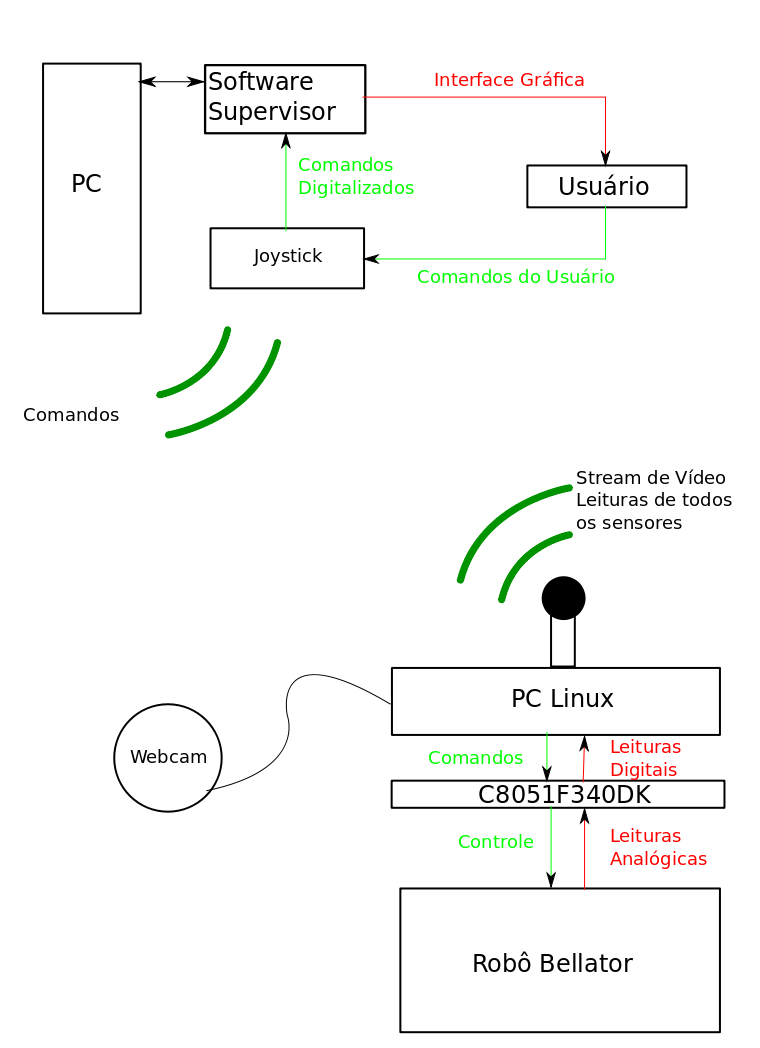
\includegraphics[width=0.8\textwidth]{./figs/diagsis.png}
	\caption[Diagrama original do Bellator]{Diagrama original do projeto Bellator, retirado da monografia do mesmo.}
	\fonte{\cite{BELLATOR}}
	\label{fig:diagsis}
\end{figure}

A partir da figura \ref{fig:diagsis}, o funcionamento do projeto Bellator pode ser explicado. A camada de baixo n�vel � composta pelo rob� Bellator, equipado com dois motores el�tricos Bosch FPG 12V, cinco sensores de dist�ncia ``2Y0A02F98"~ da Sharp, uma bateria Unybatt 12V-7,2 Amp�re hora, duas pontes H e a placa microcontrolada C8051F340, capaz de ler e converter leituras de tens�o anal�gicas dos sensores do rob� bem como produzir sinais de controle para os motores do rob�. Esta placa est� conectada � camada de alto n�vel, composta por um PC Embarcado VIA EPIA ME60000 Mini-ITX com sistema operacional Linux, atrav�s de uma conex�o serial. Utilizando-se de um protocolo de comunica��o, esse PC embarcado envia comandos de movimenta��o para a camada de baixo n�vel (conex�o serial) e recebe as leituras dos sensores obtidas pela camada de baixo n�vel. O PC embarcado tamb�m comunica-se com a camada supervis�ria para receber comandos de movimenta��o do usu�rio e enviar as leituras dos sensores para o mesmo (comunica��o sem fio). Al�m disso, o PC embarcado envia para a camada supervis�ria, tamb�m via comunica��o sem fio, um stream de v�deo gerado por uma webcam Genius iLook 316. Finalmente, o software supervisor remoto, executado em um PC com m�quina virtual Java, fornece as informa��es recebidas da camada de alto n�vel para o usu�rio, permitindo-o tomar decis�es sobre a locomo��o do rob�. O software tamb�m recebe comandos de movimenta��o do usu�rio, gerados em um Joystick do videogame Sony Playstation 2, enviando-os para a camada de alto n�vel pela mesma conex�o. Ao receber os comandos de movimenta��o, a camada de alto-n�vel simplesmente os repassa para a camada de baixo n�vel, respons�vel pela efetiva��o dos comandos, alterando os n�veis de PWM dos motores de acordo com os comandos recebidos.

O leitor pode observar que o projeto Bellator apresenta objetivos muito distintos do projeto ``Algoritmos de Navega��o Fuzzy: Uma An�lise Qualitativa". Assim, n�o ser� feita uma descri��o detalhada de todos os componentes do projeto Bellator, entretanto, pode-se consultar a refer�ncia \cite{BELLATOR} para mais informa��es. A seguir, ser� descrito como o rob� foi recebido pela equipe e quais componentes foram reaproveitados.

\subsection{Recebimento do Rob�}
\label{sec:recrobo}

O rob� Bellator foi entregue � equipe em Abril de 2011, em uma caixa, desmontado, juntamente com toda a documenta��o dispon�vel por m�dia digital. A caixa continha os seguintes itens:

\begin{itemize}
\item Chassi do rob� Bellator com dois motores Bosch FPG12V e pontes H acoplados;
\item Cinco sensores de dist�ncia ``2Y0A02F98"~ da Sharp;
\item Duas baterias Unybatt 12V-7,2 Amp�re hora;
\item Uma placa micro-controlada C8051F340;
\item Uma placa de roteamento, produzida pelo projeto Bellator;
\item Um PC Embarcado VIA EPIA ME60000 Mini-ITX.
\end{itemize}

O chassi do rob� e seus componentes acoplados s�o a base da plataforma rob�tica a ser utilizada pela equipe e s�o cr�ticas para a execu��o desse trabalho. Os sensores de dist�ncia s�o essenciais para a localiza��o de obst�culos, fornecendo informa��es cruciais para determina��o das a��es a serem tomadas. A placa microcontrolada tamb�m � um recurso cr�tico, pois � o componente respons�vel por todo o controle de baixo n�vel do rob� (acionamento dos motores, convers�o das leituras dos sensores, contagem dos pulsos dos encoders). As baterias s�o um recurso necess�rio e de f�cil aquisi��o, ao contr�rio dos outros componentes citados.

Alguns itens mencionados na se��o anterior, referentes ao projeto Bellator, n�o foram recebidos ou n�o ser�o utilizados nesse trabalho. A webcam e joystick n�o foram entregues pois n�o ser�o necess�rios, visto que um sistema de navega��o aut�nomo n�o � necess�rio o joystick e esse trabalho n�o abordar� navega��o atrav�s de imagem de v�deo. A placa de roteamento entregue ser� utilizada nos testes dos componentes, visto que � essencial para o funcionamento do rob�. Esta placa ser� reprojetada e reconstru�da. O PC embarcado foi entregue destitu�do de qualquer documenta��o. Al�m disso, como o novo objetivo do rob� n�o necessita de comunica��o sem fio e n�o utilizar� stream de v�deo, motivo principal para a utiliza��o deste PC no projeto Bellator~\cite{BELLATOR}, a equipe optou por descartar este recurso do projeto e utilizar outra placa mais simples e menor, que ser� descrita em detalhes na se��o \ref{chap:esprob}.

A documenta��o dispon�vel � equipe, produzida durante o projeto Bellator, descreve em detalhes os componentes de hardware dessa plataforma rob�tica, o software de controle supervis�rio e a camada de baixo n�vel, ou seja, o software da placa C8051F340~\cite{BELLATOR}. Essa documenta��o ser� utilizada como refer�ncia para o reaproveitamento do projeto Bellator nesse trabalho, com exce��o da documenta��o referente ao software de controle supervis�rio, que n�o ser� utilizado. O processo de reconstru��o e adapta��o da plataforma rob�tica � descrito em detalhes no cap�tulo \ref{chap:desenv}.

\subsection{Considera��es}
A possibilidade de reaproveitamento parcial do projeto Bellator e o recebimento desse material consistiram uma importante etapa nesse trabalho. A plataforma Bellator � uma op��o de recurso ao apoio do estudo qualitativo proposto nesse TCC.

%---------- Especifica��es do hardware do rob� ----------
\section{Especifica��es do Rob�}
\label{sec:esprob}

Esta se��o visa descrever a composi��o de \emph{hardware} do rob�
Bellator ap�s a reconstru��o e adequa��o do mesmo. Essa decri��o
inclui a apresenta��o dos sensores infravermelhos, enconders
�pticos, placa microcontrolada C8051F340DK, placa TS-7260, placa de roteamento e a apresenta��o do produto final, ou seja, o rob� montado.

\subsection{Sensor IR 2Y0A02F98}
\label{sec:sensores}
O sensor 2Y0A02F98 � um sensor anal�gico infravermelho e mede dist�ncias no intervalo de 20 a 150 cent�metros \cite{datasheetsensor}, sendo que os valores de tens�o de resposta do sensor seguem a curva mostrada na figura \ref{curva}. Como o valor de leitura � anal�gico, foi necess�rio que a placa C8051F340DK fosse programada para converter essa leitura em digital. O c�digo de convers�o est� de acordo com o projeto Bellator \cite{BELLATOR} e tamb�m efetua a transfer�ncia desses dados por comunica��o serial.

\begin{figure}[H]
  \centering
  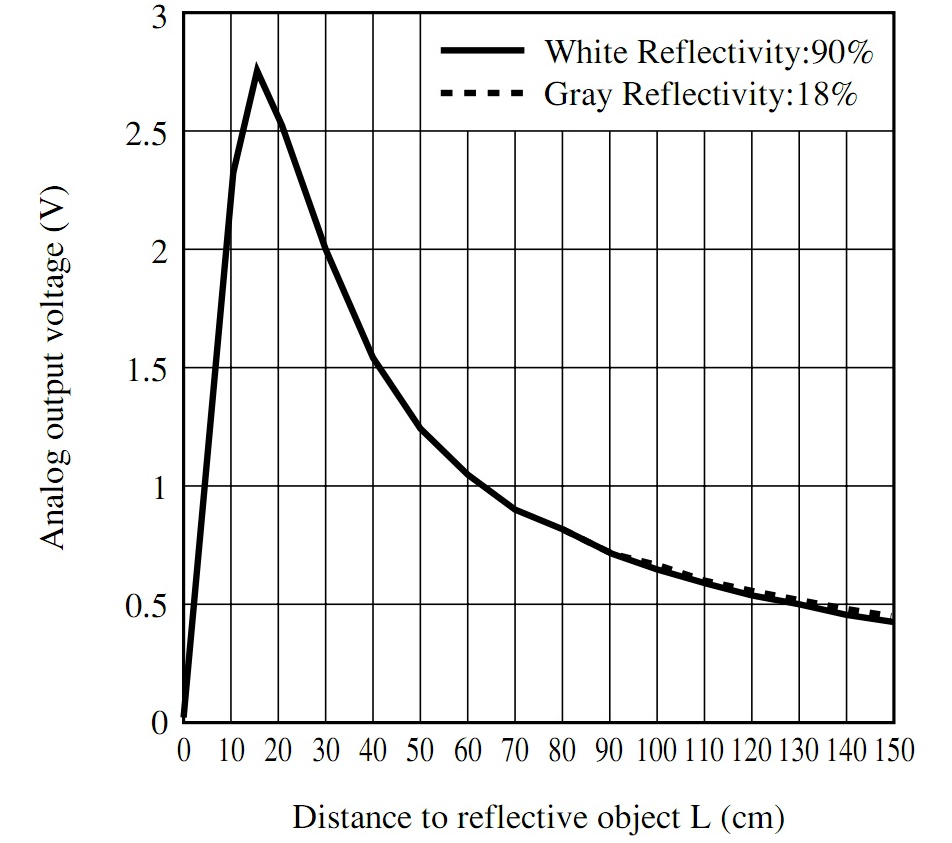
\includegraphics[width=0.5\textwidth]{./figs/curvaresp.png}
  \caption[Curva de resposta do sensor de dist�ncia]{Curva de resposta do sensor de dist�ncia.}
  \fonte{\cite{datasheetsensor}}
  \label{curva}
\end{figure}

O modelo � pouco influenciado pelas cores dos objetos refletidos, isso � devido ao m�todo de medi��o baseado em triangula��o \cite{datasheetsensor}. O sensor possui uma tens�o de alimenta��o recomendada na faixa de 4,5 a 5,5 V \cite{datasheetkit}. Como as baterias dispon�veis eram de 12 V, foi necess�ria utiliza��o de um regulador de tens�o. O c�lculo dos valores dos resistores foram baseados na equa��o \ref{eqRegulador} e o diagrama esquem�tico do regulador � mostrado na figura \ref{regulador}. Esse circuito comp�e uma das partes da placa de roteamento, conforme mostrado na se��o \ref{sec:espplacaroteamento}.

\begin{equation}
\label{eqRegulador}
V_{OUT} = 1,25V (1 + R_{2}/R_{1})
\end{equation}

\begin{figure}[H]
  \centering
  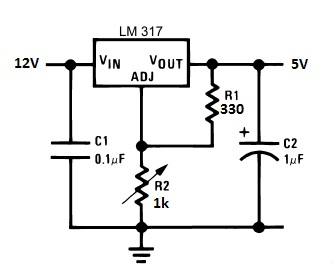
\includegraphics[width=0.5\textwidth]{./figs/regulador.jpg}
  \caption[Diagrama esquem�tico do regulador de tens�o dos sensores de dist�ncia]{Diagrama esquem�tico do regulador de tens�o dos sensores de dist�ncia.}
  \fonte{\cite{LM317}}
  \label{regulador}
\end{figure}

O modelo em quest�o � adequado ao projeto pois apresenta dimens�es compat�veis com o chassi do rob� e, como a finalidade desses sensores � auxiliar a navega��o do rob� em ambientes fechados, a faixa de resposta � suficiente para detec��o de objetos. Contudo, h� a possibilidade de, em projetos futuros, acrescentar outros tipos de sensores mais precisos voltados � medi��o de dist�ncias menores.

\subsection{Encoder �ptico HEDS-9700}
\label{sec:heds9700}
O \emph{encoder} �ptico HEDS-9700 � um circuito capaz de gerar uma onda quadrada � medida que um \emph{encoder} de quadratura � rotacionado \cite{HEDS9700}. A curva de resposta desse sensor � ilustrada na figura \ref{fig:HEDS-9700}. Nessa figura s�o ilustrados dois canais A e B, havendo um defasamento de $\phi$ entre os sinais. Nesse projeto, foi utilizado o sinal de apenas um dos canais, pois a informa��o desejada era simplesmente a contagem de pulsos gerada por cada encoder. O \emph{encoder} de quadratura utilizado na plataforma rob�tica est� fixado no eixo de cada roda e apresenta 1800 pulsos por volta. A placa C8051F340DK foi programada para contar esses pulsos e fornecer uma medida odom�trica para realimenta��o da velocidade. Essa programa��o � descrita na se��o \ref{sec:codmicro} e permite ajustar a velocidade das rodas de forma independente. Como a placa de roteamento do projeto de oficinas \cite{BELLATOR} n�o foi projetada para tratar o sinal deste \emph{encoder}, foi projetada uma nova vers�o dessa placa, descrita na se��o \ref{sec:espplacaroteamento}.

\begin{figure}[H]
  \centering
  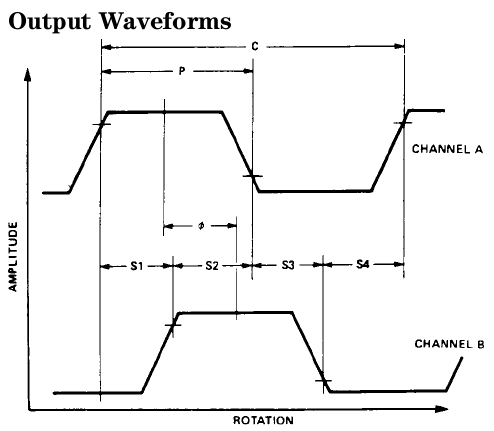
\includegraphics[width=0.5\textwidth]{./figs/HEDS-9700.png}
  \caption[Formas de onda de sa�da do \emph{encoder} �ptico]{Formas de onda de sa�da do encoder �ptico.}
  \label{fig:HEDS-9700}
  \fonte{\cite{HEDS9700}}
\end{figure}

\subsection{C8051F340DK}
\label{sec:C8051F340DK}

O C8051F340 � uma unidade microcontroladora (MCU) equipada com um n�cleo da fam�lia 8051 e v�rios dispositivos perif�ricos dispostos em uma placa de circuito impresso. As especifica��es dessa unidade foram retiradas do relat�rio do projeto Bellator \cite{BELLATOR}. O diagrama em blocos do kit � apresentado na figura \ref{dbloc}. A C8051F340 possui as seguintes caracter�sticas \cite{datasheetkit}:

\begin{itemize}
  \item Conversor ADC 10 bits de at� 200 ksps (amostras por segundo);
  \item Dois comparadores;
  \item \emph{Brown-out Reset} e \emph{Power-on Reset};
  \item Tens�o de Refer�ncia interna;
  \item Porta USB 2.0;
  \item Duas \emph{interfaces} seriais (UART) e uma \emph{interface} SPI;
  \item Fonte de Alimenta��o de 2.7 at� 5.25V regulada internamente;
  \item Micro-processador 8051 de at� 48 MIPS;
  \item 4352 Bytes de mem�ria RAM;
  \item 40 Portas de E/S;
  \item 4 temporizadores de 16 bits;
  \item Sele��o de \emph{clock} interno de alta ou baixa velocidade ou \emph{clock} externo.
\end{itemize}

\begin{figure}[H]
  \centering
  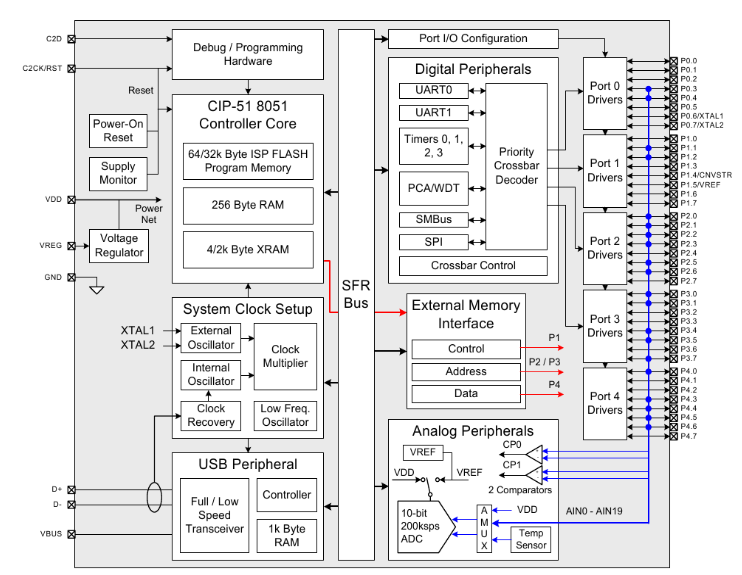
\includegraphics[width=0.8\textwidth]{./figs/dbloc.png}
  \caption[Diagrama em blocos do kit C8051F340DK]{Diagrama em blocos do kit C8051F340DK.}
  \fonte{\cite{datasheetkit}}
  \label{dbloc}
\end{figure}

\subsection{Placa TS-7260}
\label{sec:espts7260}

A placa TS-7260 � um sistema embarcado equipado com um processador ARM e sistema operacional Linux. O sistema possui perif�ricos para realiza��o de comunica��o serial, ethernet, usb, entre outros. A lista a seguir descreve os componentes relevantes para o projeto. Os dados, bem como a figura \ref{fotots}, foram retirados do \emph{datasheet} \cite{TS-7260}.

\begin{itemize}
  \item Processador ARM9 de 200MHz baseado no Cirrus EP9302
  \item 32MB de mem�ria NAND Flash
  \item 32MB de mem�ria SDRAM
  \item Consumo menor que 1 Watt mesmo em capacidade m�xima
  \item Porta Ethernet 10/100
  \item Duas portas USB 2.0
  \item Entrada de 4.5 a 20 Volts
  \item Dimens�es: 9.7 cm por 11.5cm
\end{itemize}

\begin{figure}[H]
  \centering
  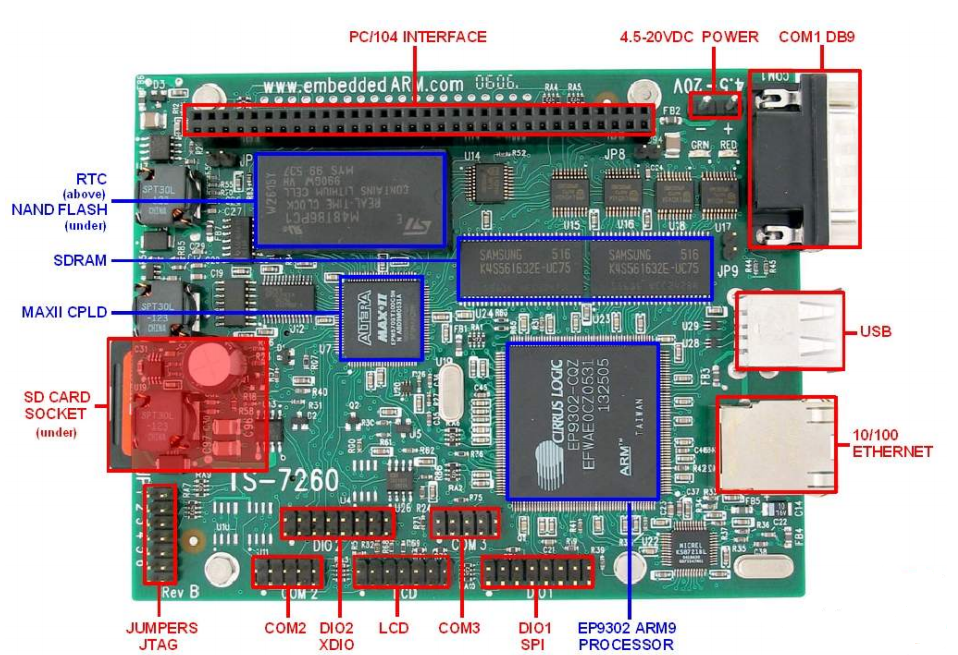
\includegraphics[width=0.8\textwidth]{./figs/fotots.png}
  \caption[Foto da placa TS-7260]{Foto da placa TS-7260.}
  \fonte{\cite{tsmanual}}
  \label{fotots}
\end{figure}

Mais informa��es sobre o sistema, bem como a documenta��o completa, est�o dispon�veis no manual da placa, dispon�vel nas refer�ncias bibliogr�ficas \cite{tsmanual}.

\subsection{Placa de Roteamento}
\label{sec:espplacaroteamento}

A placa de roteamento � um componente desenvolvido com base na placa dispon�vel do projeto Bellator \cite{BELLATOR}. Como a placa de roteamento recebida com o Bellator n�o tratava os sinais dos \emph{encoders} e estava constru�da de forma rudimentar, em uma placa universal, ela foi reprojetada e reconstru�da pela equipe. As especifica��es da placa de roteamento s�o:
\begin{itemize}
    \item Dimens�es: 5 x 9 cm;
    \item Trilhas de cobre de aproximadamente 1 mm;
    \item Regulador de tens�o LM317T: Entrada at� 40V, Sa�da 5,05V;
    \item \emph{Buffer} para PWM: 74LS244;
    \item Conectores para cabos \emph{flat}, PWM, Sensores e \emph{Encoders}.
\end{itemize}

O projeto da placa, m�todos de desenvolvimento, requisitos, entre outros ser�o descritos de forma detalhada na se��o \ref{sec:desroteamento}.

\subsection{Rob� Bellator}
\label{sec:robobellator}

O rob� Bellator, como mencionado na se��o \ref{sec:estpro}, foi reconstru�do e adaptado ao projeto. O rob� consiste de um chassi de 40 cm de largura por 50 cm de comprimento, duas rodas de tra��o e uma roda guia, conforme ilustrado na figura \ref{fig:dispsensor}. As rodas de tra��o est�o nas laterais da parte dianteira do rob� e possuem di�metro de 20 cm e largura de 4 cm. Ambas possuem o \emph{encoder} �ptico HEDS-9700, descrito na se��o \ref{sec:heds9700}, fixados nos respectivos eixos. A roda guia est� no centro da parte traseira do rob� e possui di�metro de aproximadamente 6 cent�metros e espessura de 2 cent�metros. Todas as rodas s�o da marca Schioppa e chassi do rob� permanece a 3 cm da superf�cie do solo. Com o objetivo de auxiliar a navega��o do rob� e fazer varreduras do ambiente, foram fixados cinco sensores do modelo 2Y0A02F98, descrito na se��o \ref{sec:sensores}, dispostos uniformemente nas laterais do chassi, conforme ilustra a figura \ref{fig:dispsensor}. Os outros componentes do rob� est�o listados a seguir:
\begin{itemize}
  \item[-] 2 Motores Bosch FPG 12V;
  \item[-] 2 Baterias Unybatt 12V-7,2 Amp�re-hora;
  \item[-] Duas pontes H L 298.
\end{itemize}

\begin{figure}[H]
  \centering
  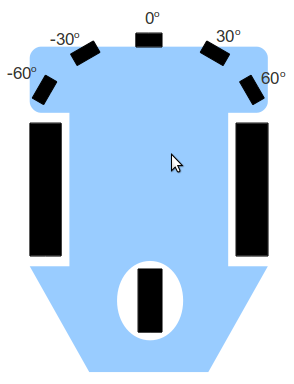
\includegraphics[width=0.3\textwidth]{./figs/dispsensor.png}
  \caption[Disposi��o dos sensores infravermelhos e rodas]{Disposi��o dos sensores infravermelhos e rodas.}
  \fonte{Autoria pr�pria}
  \label{fig:dispsensor}
\end{figure}

A plataforma transporta as placas do sistema microcontrolado C8051F340DK, descrito na se��o \ref{sec:C8051F340DK}, o sistema embarcado TS-7260, descrito na se��o \ref{sec:espts7260} e a placa de roteamento, descrita na se��o \ref{sec:espplacaroteamento}. O rob� montado pode ser visualizado na figura \ref{bellator}, que ilustra a disposi��o dos sensores infravermelhos, rodas, baterias e placas no chassi.

\begin{figure}[H]
  \centering
  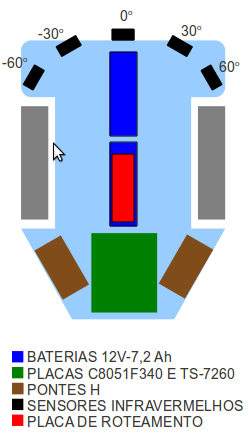
\includegraphics[width=0.3\textwidth]{./figs/bellator.png}
  \caption[Rob� Bellator montado]{Rob� Bellator montado.}
  \fonte{Autoria pr�pria}
  \label{bellator}
\end{figure}



\section{L�gica Fuzzy}
\label{sec:logfuzzy}
Esta se��o descreve os conceitos fundamentais utilizados pela equipe para o entendimento e implementa��o do algoritmo de navega��o fuzzy, descrito em detalhes na se��o \ref{sec:algfuzzy}.

\subsection{Conjuntos Fuzzy}

A teoria de conjuntos fuzzy foi elaborada inicialmente por Lofti Zadeh \cite{ZADEH}, visando explorar a possibilidade de criar um novo crit�rio de afilia��o � conjuntos. Na teoria cl�ssica de conjuntos, um elemento pode apenas pertencer ou n�o a um conjunto, sendo imposs�vel um n�vel de pertin�ncia parcial. J� em um conjunto fuzzy, isto torna-se poss�vel.
Um conjunto fuzzy pode ser definido por um conjunto de pares ordenados com o elemento e sua pertin�ncia ao conjunto fuzzy. Seja F um conjunto fuzzy e X um conjunto de objetos arbitr�rios, tem-se:

\begin{equation}
F=\{(x,f(x)),x\in X\}, f(x) = [0,1]
\end{equation}

Assim sendo, considere um conjunto ``A"~ simples que contenha tudo o que tem sabor doce. Neste conjunto uma barra de chocolate � doce da mesma forma que cana de a�ucar, visto que ambos pertencem ao conjunto, ou seja:
(barra de chocolate) $\in$ A e (cana de a�ucar) $\in$ A
Em um conjunto fuzzy B que contemple tudo o que tem sabor doce, torna-se poss�vel atribuir um n�vel de afilia��o ao conjunto atrav�s de uma fun��o de pertin�ncia f  permitindo dizer que, por exemplo, a cana de a�ucar � doce com n�vel de pertinencia 1, enquanto que a barra de chocolate � doce com n�vel de pertin�ncia 0.8, ou seja:\\*

\begin{center}
((cana de a�ucar),f(cana de a�ucar)) $\in$ B, f(cana de a�ucar) = 1\\*
((barra de chocolate),f(barra de chocolate)) $\in$ B, f(barra de chocolate) = 0.8\\*
\end{center}

Isto aproxima-se mais da forma como a cogni��o e intui��o humana funcionam, frequentemente utilizando palavras como ``mais", ``muito", ``pouco", entre outras, para definir graus de pertin�ncia a conjuntos de uma forma subjetiva.

\subsection{Vari�vel Lingu�stica}
\label{varling}

Uma aplica��o direta de conjuntos fuzzy � a defini��o de vari�veis lingu�sticas. \cite{PEDRYCZ}
Considerando que uma vari�vel \emph{x} pode assumir um valor qualquer dentro de um dado conjunto A, pode-se definir uma vari�vel lingu�stica como uma vari�vel cujo conjunto A de valores poss�veis � um conjunto de termos lingu�sticos, tais como: alto, baixo, curto, longo, entre outros. Pode-se estender este conceito associando cada termo lingu�stico poss�vel de uma vari�vel lingu�stica a um conjunto fuzzy.

Para entender esta defini��o, considere a vari�vel lingu�stica Temperatura (T) composta pelos termos lingu�sticos frio, morno e quente:
\begin{equation}
T = \{frio, morno, quente\}
\end{equation}
Considere tamb�m os seguintes conjuntos fuzzy:
\begin{equation}
	\begin{array}{lcl}
		F & = & \{(t,f(t)),t \in \mathbb{R}\} \\
		M & = & \{(t,m(t)),t \in \mathbb{R}\} \\
		Q & = & \{(t,q(t)),t \in \mathbb{R}\} \\
	\end{array}
\end{equation}
sendo \emph{\mbox{f(t), m(t) e q(t)}} fun��es de pertin�ncia, respectivamente, aos conjuntos fuzzy \emph{\mbox{F, M e Q}}, com valores de pertin�ncia pertencentes ao intervalo [0,1] e \emph{t} uma vari�vel representando a temperatura em um material qualquer. Considere ainda a associa��o dos conjuntos fuzzy \emph{\mbox{F, M e Q}} aos termos lingu�sticos frio, morno e quente, respectivamente. Neste cen�rio, um dado valor para a vari�vel \emph{t} pode ser traduzido em um valor equivalente para a vari�vel lingu�stica \emph{T}, dependendo apenas da defini��o das fun��es de pertin�ncia \emph{\mbox{f(t), m(t) e q(t)}}.

\begin{figure}[!htb]
	\centering
	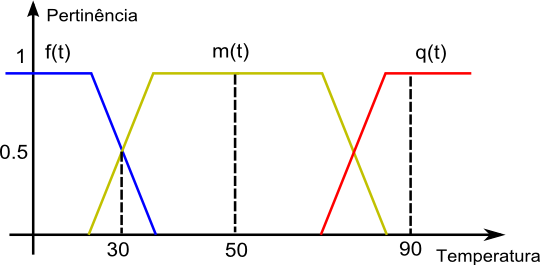
\includegraphics[width=0.8\textwidth]{./figs/fuzzygraph.png}
	\caption[Exemplo de Pertin�ncias Fuzzy]{Fun��es de Pertin�ncia f(t), m(t), q(t).}
	\label{fig:fuzzygraph}
\end{figure}

Se considerarmos, por exemplo, a defini��o gr�fica para as fun��es \emph{\mbox{f(t), m(t) e q(t)}} dada na figura \ref{fig:fuzzygraph}, e tr�s valores de temperatura, \emph{\mbox{t1 = 30, t2 = 50 e t3 = 90}}, temos que os valores correspondentes de temperatura para a vari�vel lingu�stica T s�o \mbox{T1 = (0.5 frio, 0.5 morno, 0.0 quente)}, \mbox{T2 = (0.0 frio, 1.0 morno, 0.0 quente)} e \mbox{T3 = (0.0 frio, 0.0 morno, 1.0 quente)}, respectivamente. Ou seja, informalmente, a temperatura t1 representa que o material est� ``meio frio"~ e ``meio morno"~, a temperatura t2 indica que est� ``morno"~ e a temperatura t3, por sua vez, ``quente"~. Este processo de convers�o para uma vari�vel lingu�stica � comumente chamado de ``fuzzifica��o".


\subsection{Controle Fuzzy}
\label{sec:fuzzycontrol}
Ap�s definidas as vari�veis lingu�sticas, conjuntos fuzzy e suas fun��es de pertin�ncia, descritas na se��o \ref{varling}, pode-se construir um controle fuzzy baseado em um conjunto de regras de infer�ncia.

Regras de infer�ncia sobre conjuntos fuzzy podem ser categorizadas como uma generaliza��o do \emph{modus ponens} bin�rio. Em l�gica bin�ria, dada regra ``se X ent�o Y", onde X e Y s�o vari�veis bin�rias, a partir do momento que a premissa, representada pela vari�vel X, assume valor l�gico verdadeiro, a conclus�o, dada por Y, � verdadeira tamb�m. Em l�gica fuzzy, o mesmo racioc�nio � valido, por�m X e Y s�o vari�veis lingu�sticas, e as regras de infer�ncia s�o definidas a partir dos valores que estas vari�veis lingu�sticas podem assumir, permitindo inclusive ativa��o parcial de regras de infer�ncia. Extendendo o exemplo das temperaturas, apresentado na se��o \ref{varling}, imagine que deseja-se controlar a velocidade de um \emph{cooler} de processador, de acordo com a temperatura que este se encontra, utilizando um controle fuzzy. As regras de infer�ncia para este controle podem ser, por exemplo:
\begin{center}
    Se \emph{morno} ent�o \emph{medio}\\*
    Se \emph{quente} ent�o \emph{forte}
\end{center}
Sendo ``medio"~ e ``forte"~ valores poss�veis da vari�vel lingu�stica Velocidade (V), que controla a velocidade do \emph{cooler}, com ``medio"~ correspondendo a fun��o de pertin�ncia vm e ``forte"~ correspondendo a vf, apresentados na figura \ref{fig:defuzzygraph}:

\begin{figure}[!htb]
	\centering
	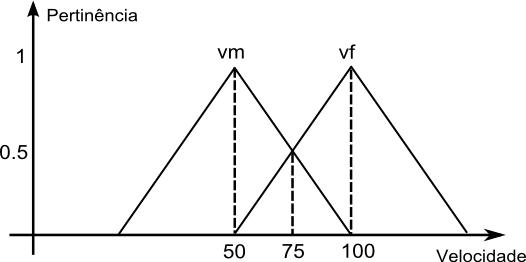
\includegraphics[width=0.8\textwidth]{./figs/defuzzygraph.png}
	\caption[Exemplo de Pertin�ncias Fuzzy - Defuzzifica��o]{Fun��es de Pertin�ncia vm e vf.}
	\label{fig:defuzzygraph}
\end{figure}

De acordo com estas regras de infer�ncia, se a temperatura \emph{fuzzificada} for inteiramente fria, nenhuma regra ser� ativada e a velocidade do \emph{cooler} ser� nula. Por�m, se a temperatura for maior que a m�nima necess�ria para come�ar a ser classificada como morna, haver� ativa��o integral ou parcial de uma ou ambas as regras de infer�ncia. Neste caso, � necess�rio determinar o grau de ativa��o de cada uma das regras e produzir uma sa�da que contemple estes graus de ativa��o, que � o processo inverso � \emph{fuzzifica��o}, a \emph{defuzzifica��o}. Um destes m�todos � a m�dia do m�ximo, que consiste da m�dia ponderada dos m�ximos de cada valor fuzzy de sa�da, com os pesos correspondendo �s ativa��es das regras de infer�ncia. Considerando novamente o exemplo do controle de velocidade de um \emph{cooler} e considerando que, em um determinado momento, a temperatura est� ``meio morno"~ e ``meio quente"~, ou seja, 0.5 de pertin�ncia � classe ``morno"~ e a classe ``quente"~, ambas as regras ser�o ativadas igualmente e a velocidade do \emph{cooler} ser�:
\begin{equation}
v = \frac{\left( 0.5*50 + 0.5*100 \right ) } {1} = 75
\end{equation}

\subsection{Considera��es}

O conceito de incerteza introduzido pela L�gica Fuzzy permite a modelagem de sistemas com problemas de decis�o cujas vari�veis s�o din�micas, reduzindo a influencia de ru�dos e possibilitando a constru��o de um sistema de infer�ncias an�logo � cogni��o humana. O problema de navega��o rob�tica � altamente din�mico, pois as decis�es s�o tomadas sob a influ�ncia de v�rios sensores simultaneamente, todos pass�veis de ru�do, e a abordagem Fuzzy � uma op��o plaus�vel para trat�-lo.

\section{Mapas Cognitivos Fuzzy}
\label{sec:fcm}
Esta se��o tem como objetivo explicar o que s�o mapas cognitivos fuzzy, tamb�m conhecidos como FCM (Fuzzy Cognitive Maps), abordando o conceito, a estrutura, as propriedades e vantagens desse modelo, apresentar os passos para contru��o de um FCM e apresentar exemplos, que descrevem o uso em situa��es reais.

O modelo FCM � abordado na tese de doutorado de \cite{FCMENDONCA}. Mapas cognitivos s�o diagramas que representam liga��es entre palavras, id�ias, tarefas ou outros itens ligados a um conceito central, dispostos radialmente, intuitivamente e de acordo com a import�ncia de cada conceito. Cren�as ou afirma��es a respeito de um dom�nio de conhecimento limitado s�o expressas por palavras ou express�es lingu�sticas interligadas por rela��es de causa e efeito, que possibilitam predizer as consequ�ncias que essa organiza��o implica ao universo representado. O mapa cognitivo fuzzy � gerado quando se incluem a essa estrutura incertezas atrav�s da l�gica Fuzzy.

\begin{figure}[!htb]
    \centering
    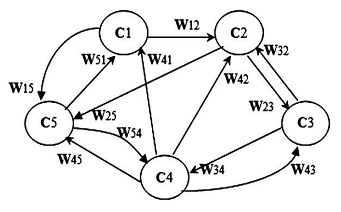
\includegraphics[width=0.5\textwidth]{./figs/fcm.png}
    \caption[Exemplo de um FCM]{Exemplo de um FCM (grafo).}
    \fonte{\cite{FCMENDONCA}}
    \label{fig:fcm}
\end{figure}

A estrutura de um FCM � um grafo direcionado, figura \ref{fig:fcm}, em que os valores num�ricos s�o vari�veis ou conjuntos fuzzy, os ``n�s"~ s�o conceitos lingu�sticos, representados por conjuntos fuzzy e cada ``n�"~ � associado a outros n�s atrav�s de conex�es (relacionamentos), a cada qual est� associado um peso num�rico, que representa a vari�vel fuzzy relacionada ao n�vel de causalidade entre os conceitos. De acordo com \cite{MENDONCA}, um FCM suporta diversos tipos de conceitos e relacionamentos:

\begin{itemize}
    \item Conceito de n�vel: Esse conceito pode pode ser representado por um valor absoluto;
    \item Conceito de varia��o: Esse tipo de conceito representa a varia��o de um valor no tempo;
    \item Conceitos de entradas: Esses conceitos recebem um valor de entrada e podem interagir com outros conceitos;
    \item Conceitos de sa�da ou de decis�o: Esses conceitos representam o resultado das infer�ncias do FCM e n�o interagem com outros conceitos;
    \item Rela��es causais: Essas conex�es representam as rela��es de causa e efeito entre os conceitos e s�o calculadas atrav�s da matriz de pesos (matriz W);
    \item Declara��es condicionais: Esses elementos s�o as rela��es causais expressas na forma de regras \emph{se-ent�o} e s�o atualizadas temporalmente.
\end{itemize}

Na figura \ref{fig:fcm}, os conceitos (C1 a C5) podem ser atualizados atrav�s da intera��o com outros conceitos por meio das rela��es causais ($w_{i,j}$) e com seu pr�prio valor. A matriz \ref{fcm-matrix} representa o peso das rela��es causais entre os conceitos e podem ser atualizados atrav�s da equa��o \ref{fcm-update}. Esta descreve a evolu��o do FCM, na qual j � o contador das itera��es, n � o n�mero de n�s do grafo, $W_{ji}$ � o peso do arco que conecta o conceito $C_j$ ao conceito $C_i$, $A_i$ e $A_i^{anterior}$ s�o o valor do conceito $C_i$ na itera��o atual e anterior, respectivamente, e a fun��o f \ref{sigmoide} � uma fun��o do tipo sigm�ide.

\begin{equation}\label{fcm-matrix}
    w_{i,j}=\left(
       \begin{array}{ccccc}
         0 & w_{12} & 0 & 0 & w_{15} \\
         0 & 0 & w_{23} & 0 & w_{25} \\
         0 & w_{32} & 0 & w_{34} & 0 \\
         w_{41} & 0 & w_{43} & 0 & w_{45} \\
         w_{51} & 0 & 0 & w_{54} & 0 \\
       \end{array}
     \right)
\end{equation}

\begin{equation}\label{fcm-update}
A_i=f(\sum_{\substack{j=1 \\ j\neq i}}^{n} A_j \times W_{ji})+A_i^{anterior}
\end{equation}

\begin{equation}\label{sigmoide}
f(x)=\frac{1} {1+e^{-\lambda x}}
\end{equation}

Em \cite{KOSKO}, s�o apresentados os seguintes passos para constru��o de um FCM cl�ssico:

\begin{itemize}
\item Passo 1 - Identifica��o dos conceitos e das suas interconex�es ou rela��es
determinando a natureza (positiva, negativa ou neutra) das rela��es causais entre
conceitos;
\item Passo 2 - Aquisi��o de dados iniciais, atrav�s de pondera��o de opini�o de
especialistas e ou an�lise do sistema de equa��es, quando se conhece o modelo
matem�tico;
\item Passo 3 - Apresenta��o dos dados referentes � opini�o dos diversos especialistas a
um sistema l�gico fuzzy que tem como sa�da os valores dos pesos do FCM;
\item Passo 4 - Tratamento da informa��o, adapta��o e ou otimiza��o do FCM
inicialmente proposto, ajustando suas respostas �s sa�das desejadas;
\item Passo 5 - Valida��o do FCM ajustado nas condi��es de opera��o do sistema ou
processo modelado.
\end{itemize}

Um FCM apresenta as propriedades de elasticidade e estabilidade, sendo que a elasticidade, ou auto organiza��o, � a capacidade de refor�ar ou enfraquecer o peso das rela��es causais e a estabilidade � a capacidade de o mapa evoluir, estabilizando-se em um ponto fixo ou ap�s um n�mero m�ximo de itera��es. Uma vantagem do FCM � a modularidade, a qual permite que um problema complexo seja representado por v�rios mapas modulares e outra vantagem � que os pesos das rela��es causais e dos conceitos podem ser obtidos via treinamento a partir dos dados hist�ricos do sistema ou atrav�s de um algoritmo adaptativo, que atualiza os pesos constantemente.

\begin{figure}[!htb]
    \centering
    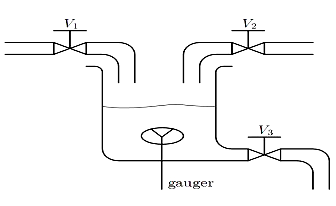
\includegraphics[width=0.5\textwidth]{./figs/fcm-exemplo-planta.png}
    \caption[Aplica��o do FCM em processo industrial]{Aplica��o do FCM em processo industrial.}
    \fonte{\cite{GROUMPOS}}
    \label{fig:fcm-exemplo-planta}
\end{figure}

Em \cite{GROUMPOS} os mapas cognitivos fuzzy s�o aplicados no controle de processos industriais. Um exemplo de aplica��o � mostrado na figura \ref{fig:fcm-exemplo-planta}, na qual � ilustrado um tanque com duas v�lvulas de entrada (V1 e V2) para diferentes tipos de l�quidos, um misturador, uma v�lvula de sa�da (V3) para o l�quido misturado e um medidor de massa espec�fica (G) que mede a quantidade de l�quido produzida. As v�lvulas V1 e V2 introduzem dois l�quidos diferentes. Durante a mistura, o medidor de massa espec�fica verifica quando o produto atingiu o ponto adequado e, desse modo, a v�lvula V3 � ativada e o produto da mistura � esvaziado. Analisando-se o problema, os seguintes conceitos podem ser definidos:

\begin{itemize}
\item Conceito 1: Volume de l�quido no tanque, o qual depende do estado das v�lvulas V1, V2 e V3;
\item Conceito 2: Estado da v�lvula 1 (fechada, aberta ou parcialmente aberta);
\item Conceito 3: Estado da v�lvula 2 (fechada, aberta ou parcialmente aberta);
\item Conceito 4: Estado da v�lvula 3 (fechada, aberta ou parcialmente aberta);
\item Conceito 5: Valor de massa espec�fica do l�quido medido pelo sensor G.
\end{itemize}

O controlador do processo deve manter as vari�veis V e G, sendo V o volume e G a massa especifica do produto no tanque, dentro das faixas de opera��o $[V_{min}, V_{max}]$ (equa��o \ref{lim-V}) e $[G_{min}, G_{max}]$ (equa��o \ref{lim-G}), respectivamente.

\begin{equation}\label{lim-V}
V_{min}<V<V_{max}
\end{equation}

\begin{equation}\label{lim-G}
G_{min}<G<G_{max}
\end{equation}

Interligando-se os conceitos atrav�s de rela��es de causa e efeito, o FCM da figura \ref{fig:fcm-exemplo-fcm} foi constru�do.

\begin{figure}[!htb]
    \centering
    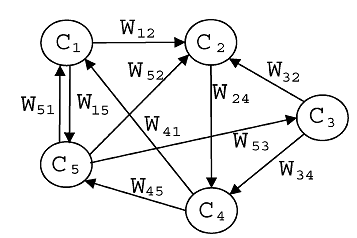
\includegraphics[width=0.5\textwidth]{./figs/fcm-exemplo-fcm.png}
    \caption[Mapa Cognitivo Fuzzy]{FCM do controlador.}
    \fonte{\cite{GROUMPOS}}
    \label{fig:fcm-exemplo-fcm}
\end{figure}

 Analisando-se o conhecimento dos especialistas, os pesos das rela��es s�o dados pelas inequa��es \ref{peso-1} a \ref{peso-8}.

\begin{equation}\label{peso-1}
-0,50<w_{12}<0,30
\end{equation}
\begin{equation}\label{peso-2}
-0,40<w_{13}<0,20
\end{equation}
\begin{equation}\label{peso-3}
0,20<w_{15}<0,40
\end{equation}
\begin{equation}\label{peso-4}
0,30<w_{21}<0,40
\end{equation}
\begin{equation}\label{peso-5}
0,40>w_{31}<0,50
\end{equation}
\begin{equation}\label{peso-6}
-1,0<w_{41}<0,80
\end{equation}
\begin{equation}\label{peso-7}
0,50<w_{52}<0,70
\end{equation}
\begin{equation}\label{peso-8}
0,30<w_{54}<0,40
\end{equation}

O controlador do processo foi executado e, ap�s a estabiliza��o, obtiveram-se os pesos da matriz \ref{W-matrix} e os valores dos conceitos da matriz \ref{A-matrix}. Os limites das equa��es \ref{lim-V} e \ref{lim-G} s�o reajustados para os valores correspondentes �s equa��es \ref{lim-V-adj} e \ref{lim-G-adj}, respectivamente, correspondendo ao ponto de opera��o desejado.

\begin{equation}\label{W-matrix}
    W^{inicial}=\left(
       \begin{array}{ccccc}
         0,00 & -0,40 & -0,25 & 0,00 & 0,30 \\
         0,36 & 0,00 & 0,00 & 0,00 & w0,00 \\
         0,45 & 0,00 & 0,00 & 0,00 & 0,00 \\
         -0,90 & 0,00 & 0,00 & 0,00 & 0,00 \\
         0,00 & 0,60 & 0,00 & 0,30 & 0,00 \\
       \end{array}
     \right)
\end{equation}

\begin{equation}\label{A-matrix}
    A^{inicial}=\left(
       \begin{array}{ccccc}
         0,10 & 0,45 & 0,39 & 0,04 & 0,01 \\
       \end{array}
     \right)
\end{equation}

\begin{equation}\label{lim-V-adj}
0,68<V<0,70
\end{equation}

\begin{equation}\label{lim-G-adj}
0,78<G<0,85
\end{equation}

Nesse exemplo, a estabiliza��o (ou sintonia) foi realizada atrav�s de tr�s m�todos: RNA (Rede Neural Artificial), AG (Algoritmo Gen�tico) e PSO (Particle Swarm Optimization ou Otimiza��o por Enxame de Part�culas).

Outra aplica��o � descrita no artigo \cite{MENDONCA}, na qual a abordagem FCM � empregada em navega��o rob�tica. Nesse artigo, um modelo de FCM novo � implementado para suportar as condi��es din�micas dos sistemas de navega��o, nas quais os valores das rela��es causais s�o modificados dinamicamente atrav�s da ocorr�ncia de eventos especiais. Os autores do artigo chamaram esse modelo de ED-FCM (Event-Driven Fuzzy Cognitive Map).

\begin{figure}[!htb]
    \centering
    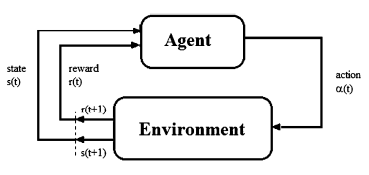
\includegraphics[width=0.5\textwidth]{./figs/reinforcement.png}
    \caption[Algoritmo de aprendizado por refor�o]{Algoritmo de aprendizado por refor�o.}
    \fonte{\cite{MENDONCA}}
    \label{fig:reinforcement-alg}
\end{figure}

O ajuste dos pesos das rela��es causais � efetuado por um algoritmo de aprendizado por refor�o, conforme ilustra a figura \ref{fig:reinforcement-alg}, e permite que o rob� (agente) aprenda diretamente atrav�s de sua intera��o com o ambiente. A cada instante de tempo t, o agente estabelece, por meio de seus sensores, um estado st e, de acordo com suas regras, determina uma a��o at a ser efetuada pelos atuadores. Essa a��o causa uma transi��o para o estado $s_{t+1}$ e o ambiente retorna uma medida de refor�o $r_{t+1}$, que pode ser uma recompensa (caso a a��o seja boa) ou uma puni��o (caso a a��o seja ruim).

\begin{figure}[!htb]
    \centering
    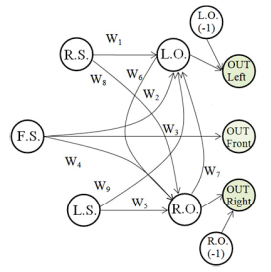
\includegraphics[width=0.5\textwidth]{./figs/fcm-robot.png}
    \caption[FCM do comportamento reativo do rob�]{FCM do comportamento reativo do rob�.}
    \fonte{\cite{MENDONCA}}
    \label{fig:fcm-robot}
\end{figure}

O FCM descreve o comportamento reativo do rob� (figura \ref{fig:fcm-robot}), no qual a leitura dos sensores de dist�ncia (esquerdo, frontal e direito) levam a uma a��o imediata que interfere no movimento. Os conceitos RS, FS e LS representam as leituras dos sensores, os conceitos LO e RO representam as decis�es de virar � esquerda ou virar � direita, respectivamente,  decis�es anteriores, representadas pelos conceitos LO(-1) e RO(-1), exercem influ�ncia sobre as decis�es atuais e a sa�da do algoritmo � representada pelos conceitos \emph{Out Left}, \emph{Out Front} e \emph{Out Right}. As rela��es causais do mapa s�o descritas na tabela \ref{tab:causal-relations} e as regras de a seguir determinam o comportamento do mapa:

\begin{enumerate}
\item SE a intensidade do sensor frontal (FS) for maior que um limiar m�dio ENT�O $W_{lim}$ aplicado para computar o relacionamento $w_3$ � o valor m�ximo de $WF_{max}$;
\item SE a intensidade do sensor frontal (FS) for menor que um limiar m�nimo ENT�O $W_{lim}$ aplicado para computar o relacionamento $w_3$ � o valor m�nimo de $WF_{min}$;
\item SE a intensidade do sensor direito (RS) for maior que um limiar m�dio ENT�O $W_{lim}$ aplicado para computar o relacionamento $w_1$ � o valor m�ximo de $WR_{max}$;
\item SE a intensidade do sensor direito (RS) for menor que um limiar m�nimo ENT�O $W_{lim}$ aplicado para computar o relacionamento $w_1$ � o valor m�nimo de $WR_{min}$;
\item SE a intensidade do sensor esquerdo (LS) for maior que um limiar m�dio ENT�O $W_{lim}$ aplicado para computar o relacionamento $w_5$ � o valor m�ximo de $WL_{max}$;
\item SE a intensidade do sensor direito (LS) for menor que um limiar m�nimo ENT�O $W_{lim}$ aplicado para computar o relacionamento $w_5$ � o valor m�nimo de $WL_{min}$.
\end{enumerate}

\begin{table}[htb!]
	\centering
	\caption[Rela��es causais do controlador do rob�]{Rela��es causais do controlador do rob�.}		
	\begin{tabular}[!htb]{ l l l l }
	  \hline
	  Rela��o causal & Descri��o & Efeito & Intensidade \\
	  \hline
	  $w_1$ & Sensor direito (RS) influencia a sa�da esquerda (LO) & Positivo & Forte \\
	  $w_2$ & Sensor frontal (FS) influencia a sa�da esquerda (LO) & Positivo & M�dio \\
	  $w_3$ & Sensor frontal (FS) influencia a sa�da frontal (FO) & Positivo & Forte \\
	  $w_4$ & Sensor frontal (FS) influencia a sa�da direita (RO) & Positivo & M�dio \\
	  $w_5$ & Sensor esquerdo (LS) influencia a sa�da direita (RO) & Positivo & Forte \\
	  $w_6$ & Sensor esquerdo (LS) influencia a sa�da direita (RO) & Negativo & Fraco \\
	  $w_7$ & Sensor direito (RS) influencia a sa�da esquerda (LO) & Negativo & Fraco \\
	  $w_8$ & Sensor direito (RS) influencia a sa�da direita (RO) & Negativo & Fraco \\
	  $w_9$ & Sensor esquerdo (LS) influencia a sa�da esquerda (LO) & Negativo & Fraco \\
	  \hline  	
	\end{tabular}
	\fonte{\cite{MENDONCA}}
	\label{tab:causal-relations}
\end{table}

Essas regras determinam a pol�tica de mudan�a de estados do mapa e os pesos dos relacionamentos s�o respons�veis pelas decis�es de o rob� virar � esquerda, acelerar ou virar � direita. Nesse contexto, o valor atual desses pesos depende da diferen�a entre os valores anteriores e o valor m�ximo admiss�vel ponderado por um fator $\gamma$ . O incremento dos pesos tamb�m leva em conta o valor da recompensa ou punic�o (r) e de um fator de aprendizagem $\alpha$ , os quais est�o associados ao algoritmo de aprendizado por refor�o escolhido, equa��o \ref{q-learning}.

\begin{equation}\label{q-learning}
w_i(k)=w_i(k-1)+\alpha \times [r+\gamma \times W_{lim}-w_i(k-1)]
\end{equation}

Por fim, nesse artigo, s�o descritos os resultados nos quais o rob�, em simula��o, foi capaz de desviar obst�culos � direita e � esquerda do mesmo ao longo da trajet�ria.

\subsection{Considera��es}
O FCM representa um problema em termos de conceitos e rela��es causais, podendo ser empregado em controladores de processos industriais ou no controle de rob�s aut�nomos. O problema do desvio de obst�culos em navega��o rob�tica p�de ser modelado, conforme o exemplo apresentado (figura \ref{fig:fcm-robot}), atrav�s de tr�s conceitos de entrada (RS, FS e LS), dois conceitos de decis�o (RO e LO), tr�s conceitos de sa�da (Right Out, Front Out e Left Out), rela��es causais, regras \emph{SE-ENT�O} e um algoritmo de aprendizado. O controlador proposto permitiu que o rob� desviasse obst�culos reagindo � leitura de sensores que medem a dist�ncia de objetos posicionados � esquerda e � direita do mesmo, concluindo-se que a abordagem FCM � adequada para esse trabalho.



\chapter{Conclus�o}

O presente trabalho de conclus�o de curso apresentou objetivos abrangentes, envolvendo desenvolvimento de hardware e software. No contexto da navega��o rob�tica, surgiu a necessidade de se utilizar um rob� real com a finalidade de se obter resultados mais significativos. Desse modo, foi elaborado um projeto cujo escopo tamb�m foi reconstruir e adequar uma plataforma rob�tica previamente dispon�vel, que � descrita na sec��o \ref{sec:estpro}, por�m que n�o estava em condi��es de uso imediato. A equipe procedeu com testes em laborat�rio de eletr�nica afim de avaliar as condi��es iniciais do rob�, conforme � descrito na sec��o \ref{sec:testecomp}. Uma an�lise de software foi efetuada e o c�digo original do microcontrolador C8051F340DK, disponibilizado como parte integrante do rob� Bellator \cite{BELLATOR}, foi avaliado e reconfigurado de acordo com as necessidades do projeto, o que � descrito em detalhes na se��o \ref{sec:codmicro}. Havendo necessidade de implementa��o de hardware, a equipe projetou e construiu uma placa de roteamento para alimentar os sensores e encoders, assim como tratar os sinais destes e os de PWM, como � descrito na se��o \ref{sec:desroteamento}. Finalmente, o hardware acoplado foi configurado e o software que executou os algortimos de navega��o foi desenvolvido, conforme a se��o \ref{sec:ts}. Com isso, a equipe concluiu a primeira parte do projeto, a qual consistiu na reconstru��o e adequa��o do rob� Bellator.

Estando a plataforma rob�tica funcional, seguiram-se o projeto e implementa��o dos algoritmos de navega��o propostos. A L�gica Fuzzy foi estudada e apresentada na se��o \ref{sec:logfuzzy} e a metodologia de Mapas Cognitivos Fuzzy (FCM) foi estudada e apresentada na se��o \ref{sec:fcm}. Com a teoria fundamentada, a equipe projetou os algoritmos e implementou-os na linguagem C++, compilados para executar no hardware acoplado, placa TS-7260. O projeto e a implementa��o dos algoritmos de navega��o Fuzzy e FCM s�o descritos em detalhes nas se��es \ref{sec:algfuzzy} e \ref{sec:algedfcm}, respectivamente. Ap�s a implementa��o, a equipe submeteu os algoritmos a uma s�rie de testes b�sicos, denominada Testes Iniciais, que serviram para fornecer a primeira realimenta��o do projeto dos algoritmos e pode ser lido na se��o \ref{sec:testesini}. Finalizados esses testes, foram elaborados testes complexos, denominados Testes Avan�ados, para estressar os sistemas de navega��o propostos e fornecer a segunda realimenta��o do projeto dos algoritmos, conforme � descri��o na se��o \ref{sec:testesavan}. Finalmente, ap�s os testes avan�ados, os algoritmos resolviam problemas complexos de navega��o, como o corredor sem sa�da e o problema de decis�o quando dois obst�culos laterais e um frontal era colocado diante do rob�, e poderiam ser usados nos testes finais, que forneceram os dados para a an�lise de resultados e foram denominados Testes Comparativos, conforme � descrito na se��o \ref{sec:testescomp}. Com isso foi conclu�do outros dois objetivos do projeto, que foram o projeto e implementa��o dos algoritmos de navega��o e a elabora��o e execu��o de uma metodologia de testes comparativos entre os algoritmos.

Para trabalhos futuros utilizando a plataforma Bellator reconstru�da, a equipe recomenda combinar sensores de ultra-som ao sensores infra vermelho, justificando isso porque os sensores de ultra-som apresentam uma faixa de opera��o cuja dist�ncia m�nima � menor que a do infra-vermelho, podendo capturar dist�ncias de 2 cm. Atualmente a dist�ncia m�nima suportada pelo sistema de navega��o � de 15 cm, com os sensores de ultra-som, os algoritmos poderiam operar em uma faixa mais abrangente. Outra sugest�o � introduzir ao sistema uma realimenta��o por b�ssola pois nesse projeto a realimenta��o odom�trica fornecida pelos encoders � utilizada para ajustar a velocidade das rodas e n�o faz uma interpreta��o da dire��o do rob�. Para tornar o rob� seguro para o manuseio, sugere-se a fixa��o dos sensores parafusando-os no chassi do Bellator e acoplando uma casca que proteja os circuitos microcontrolados. A equipe tamb�m recomenda a reconstru��o da placa de roteamento utilizando um m�todo industrial para confecc��o de placas de circuito impresso. Para os sistemas de navega��o, um trabalho futuro de grande riqueza seria introduzir ao sistema a capacidade de interpretar a posi��o do rob� em rela��o a um referencial. Com isso, o rob� seria capaz de resolver problemas nos quais este deve partir de um ponto inicial no espa�o a um ponto final, guiando-se pelos sensores para evitar colis�es e realimentar-se por um sistema de posicionamento para corrigir a traget�ria. Outro trabalho, produto deste, seria introduzir ao sistema uma mem�ria a qual pudesse mapear os obst�culos capturados pelos sensores do rob�, assim sendo, produzir-se-ia um artefato aut�nomo capaz de mapear terrenos. Outro aprimoramento da plataforma seria implementar um sistema de controle remoto por joystick, na qual uma base remota podesse pilotar o rob� via joystick. Finalmente, a equipe sugere um projeto futuro no qual seja implementado um sistema de vis�o computacional por c�mera de v�deo.

A equipe concluiu esta monografia justificando que os objetivos descritos na introdu��o, se��o \ref{rec:obj}, foram alcan�ados e est�o de acordo com os requisitos m�nimos de um curso de Engenharia de Computa��o. Os problemas encontrados na execu��o do projeto est�o associados ao escopo abrangente do mesmo, o qual envolveu o desenvolvimento de hardware e software em um projeto integrador. A subdivis�o do projeto em diversos objetivos, sendo um pr�-requisito para o outro, foi inevit�vel para alcan�ar os resultados finais. A equipe encontrou dificuldades durante a reconstru��o do rob�, configura��o da placa TS-7260, testes integrados de funcionamento do rob�, implementa��o dos algoritmos, execu��o dos testes dos algoritmos e an�lise de resultados. Durante a recontru��o, os componentes eletr�nicos foram testados isoladamente e houve riscos de haver danos, o que representaria atrasos no projeto. A placa TS-7260 apresentou complexidade para ser configurada pois n�o houve um t�cnico dispon�vel para auxiliar a equipe, a qual teve que aprender a trabalhar com esse hardware. Nos testes de integra��o da C8051F340DK e da TS-7260, que determinaram o funcionamento da plataforma rob�tica, foi exigido processos de depura��o integrados, nos quais os problemas foram isolados e corrigidos repetidas vezes. A implementa��o dos algoritmos at� a vers�o final, que foi utilizada nos testes comparativos, foi realizada paralelamente aos testes b�sicos e avan�ados, nas quais os problemas de navega��o foram detectados, isolados e corrigidos repetidas vezes. A metodologia de testes escolhida foi elaborada pela equipe e foram efetuados v�rios experimentos com registro em v�deo at� que se atingessem os resultados finais. Tendo com base os v�deos gravados e a experi�ncia em campo observada, a equipe precisou analisar os resultados, discut�-los e extrair conclus�es para finalizar o projeto, sendo que essa tarefa representou um trabalho cient�fico. 


%---------- Referencias ----------
\bibliography{reflatex} % geracao automatica das referencias a partir do arquivo reflatex.bib


%---------- Apendices (opcionais) ----------
\apendice
\chapter{Nome do Ap\^endice}

Use o comando {\ttfamily \textbackslash apendice} e depois comandos {\ttfamily \textbackslash chapter\{\}}
para gerar t\'itulos de ap\^en-dices.


% ---------- Anexos (opcionais) ----------
\anexo
\chapter{Nome do Anexo}

Use o comando {\ttfamily \textbackslash anexo} e depois comandos {\ttfamily \textbackslash chapter\{\}}
para gerar t\'itulos de anexos.

\end{document}
 